\let\negmedspace\undefined
\let\negthickspace\undefined
\documentclass[journal]{IEEEtran}
\usepackage[a5paper, margin=10mm, onecolumn]{geometry}
%\usepackage{lmodern} % Ensure lmodern is loaded for pdflatex
\usepackage{tfrupee} % Include tfrupee package

\setlength{\headheight}{1cm} % Set the height of the header box
\setlength{\headsep}{0mm}     % Set the distance between the header box and the top of the text

\usepackage{gvv-book}
\usepackage{gvv}
\usepackage{cite}
\usepackage{amsmath,amssymb,amsfonts,amsthm}
\usepackage{algorithmic}
\usepackage{graphicx}
\usepackage{textcomp}
\usepackage{xcolor}
\usepackage{txfonts}
\usepackage{listings}
\usepackage{enumitem}
\usepackage{mathtools}
\usepackage{gensymb}
\usepackage{comment}
\usepackage[breaklinks=true]{hyperref}
\usepackage{tkz-euclide} 
\usepackage{listings}
                                         
\def\inputGnumericTable{}                                 
\usepackage[latin1]{inputenc}                                
\usepackage{color}                                            
\usepackage{array}                                            
\usepackage{longtable}                                       
\usepackage{calc}                                             
\usepackage{multirow}                                         
\usepackage{hhline}                                           
\usepackage{ifthen}                                           
\usepackage{lscape}
\begin{document}


\bibliographystyle{IEEEtran}

\title{8.4.24}
\author{EE25BTECH11021 - Dhanush sagar}
% \maketitle
% \newpage
% \bigskip
\maketitle \vspace{-1cm}
\renewcommand{\thefigure}{\theenumi}
\renewcommand{\thetable}{\theenumi}
\setlength{\intextsep}{10pt} % Space between text and floats

\
\numberwithin{figure}{enumi}
\renewcommand{\thetable}{\theenumi}

\textbf{Question:}  \\
If the line $x - 1 = 0$ is the directrix of the parabola 
\[
y^2 - kx + 8 = 0,
\] 
then one of the values of $k$ is:
\begin{multicols}{4}
    \begin{enumerate}
    \item 18
    \item 8
    \item 4
    \item 14
\end{enumerate}
\end{multicols}

\textbf{Solution:}  \\
We are given the parabola 
\begin{align}
y^2 - kx + 8 = 0
\end{align}
with directrix \(x - 1 = 0\). Represent the parabola in matrix form:
\begin{align}
\vec{x}^\top V \vec{x} + 2 \vec{u}^\top \vec{x} + f = 0
\end{align}



For a conic with directrix \(\vec{n}^\top \vec{x} = c\), eccentricity \(e\) and focus \(\vec{F}\), the matrix formulas are:
\begin{align}
\vec{V} &= \|\vec{n}\|^2 I - e^2 \vec{n} \vec{n}^\top \\
\vec{u} &= c e^2 \vec{n} - \|\vec{n}\|^2 \vec{F} \\
f &= \|\vec{n}\|^2 \|\vec{F}\|^2 - c^2 e^2
\end{align}

For the parabola \(y^2 - kx + 8 = 0\), we write the matrices as
\begin{align}
\vec{V} &= \myvec{0 & 0 \\ 0 & 1}, &
\vec{u} &= \myvec{-k/2 \\ 0}, &
f &= 8
\end{align}

The directrix is \(\vec{n}^\top \vec{x} = c \implies \vec{n} = \myvec{1 \\ 0}, c = 1\), and for a parabola \(e = 1\). Then
\begin{align}
\vec{V} &= \|\vec{n}\|^2 I - e^2 \vec{n} \vec{n}^\top 
= 1 \cdot \myvec{1 & 0 \\ 0 & 1} - 1 \cdot \myvec{1\\0} \myvec{1 & 0} 
= \myvec{0 & 0 \\ 0 & 1}
\end{align}

The vector \(\vec{u}\) gives the focus:
\begin{align}
\vec{u} &= c e^2 \vec{n} - \|\vec{n}\|^2 \vec{F} \implies
\vec{F} = c \vec{n} - \vec{u} = \myvec{1 \\ 0} - \myvec{-k/2 \\ 0} = \myvec{1 + k/2 \\ 0}
\end{align}

The constant term is
\begin{align}
f &= \|\vec{n}\|^2 \|\vec{F}\|^2 - c^2 e^2 
= 1 \cdot \brak{ \myvec{1 + k/2 \\ 0}^\top \myvec{1 + k/2 \\ 0} } - 1 
= (1 + k/2)^2 - 1
\end{align}

Equating with the given \(f = 8\):
\begin{align}
(1 + k/2)^2 - 1 &= 8 \implies (1 + k/2)^2 = 9
\end{align}

Solving the matrix equation:
\begin{align}
1 + k/2 &= 3 \implies k = 4 \\
1 + k/2 &= -3 \implies k = -8
\end{align}

Hence, one of the values of \(k\) is
\begin{align}
\boxed{4}
\end{align}
\begin{figure}[H]
    \centering
    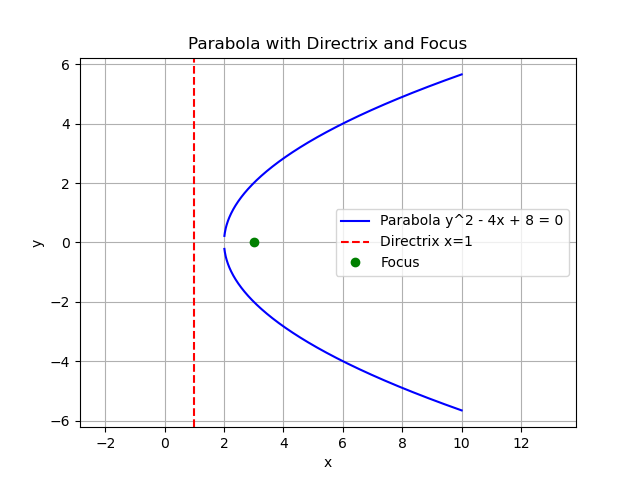
\includegraphics[width=0.8\linewidth]{Figs/Fig1.png}
    \caption{}
    \label{fig:placeholder}
\end{figure}


\end{document}


